% ============================================================================
%  ANEXĂ — o pagină la finalul lucrării, după bibliografie.
% ============================================================================


% ----------------------------------------------------------------------------
%  ACTIV: declarația de autenticitate.
%
%  ATENȚIE la numele fișierului: se folosește `declaratie-semnata.pdf`, NU
%  `declaratie.pdf`. În originalul semnat, semnătura este o adnotare (o
%  „ștampilă” lipită peste pagină), nu face parte din conținutul paginii.
%  `\includepdf` importă doar conținutul paginii, deci din original semnătura
%  ar dispărea. `declaratie-semnata.pdf` este aceeași pagină, randată la 300 DPI
%  cu semnătura încorporată definitiv.
%
%  `pages={1}`  -> inserează doar prima pagină ({1,2} pentru două, `-` pentru tot)
%  `addtotoc`   -> adaugă intrarea în cuprins FĂRĂ a tipări un titlu peste
%                  document, deci anexa ocupă o singură pagină, nu două
%  `pagecommand`-> păstrează numerotarea paginilor și pe pagina inserată
% ----------------------------------------------------------------------------

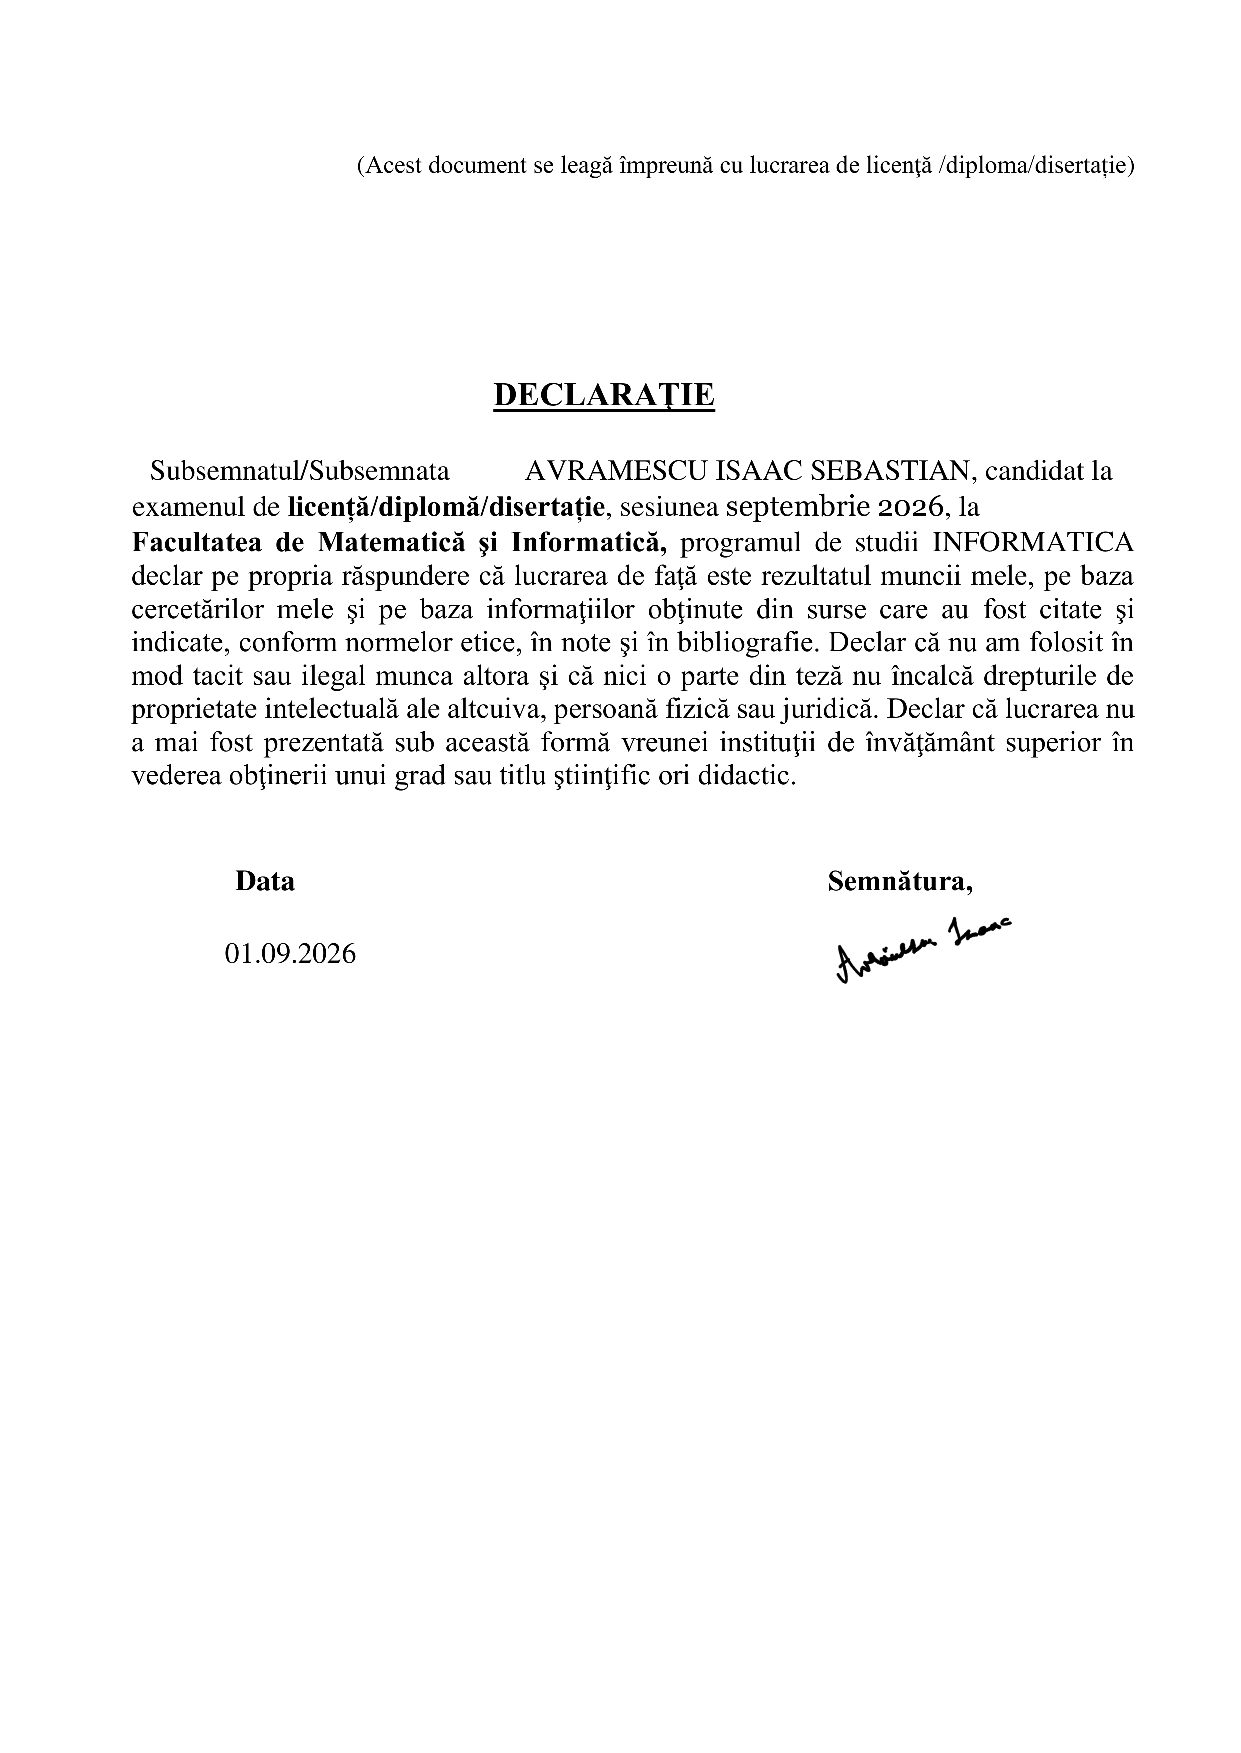
\includepdf[
    pages={1},
    addtotoc={1,chapter,0,Declarație de autenticitate,declaratie},
    pagecommand={\thispagestyle{main}}
]{declaratie-semnata.pdf}


% ----------------------------------------------------------------------------
%  ALTERNATIVĂ (comentată) — dacă vrei în schimb o IMAGINE.
%  Pune fișierul în `images/` și scrie-i numele, fără cale.
% ----------------------------------------------------------------------------

% \addcontentsline{toc}{chapter}{Anexă}
% \chapter*{Anexă}
% \begin{figure}[!ht]
%     \centering
%     \includegraphics[width=\textwidth]{numele-fisierului.png}
%     \caption{Descrierea documentului anexat}
% \end{figure}
